\documentclass[a4paper, 10pt, final]{article}
%%%%%%%%%%%%%%%%%%%%%%%%%%%%%%%%%%%%%%%%%%%%%%%%%%%%%%%%%%%%%%%%%%
% Pakker
%%%%%%%%%%%%%%%%%%%%%%%%%%%%%%%%%%%%%%%%%%%%%%%%%%%%%%%%%%%%%%%%%%
%\usepackage{a4wide}
\usepackage[danish]{babel}
\usepackage[utf8]{inputenc}
\usepackage[T1]{fontenc}
\usepackage{verbatim}
\usepackage{amsfonts}
\usepackage{amsmath}
\usepackage{amssymb}
\usepackage{mathrsfs}
\usepackage[small,bf]{caption}
\usepackage[mathcal]{euscript}
\usepackage{listings}
\usepackage{charter}
\usepackage{epsfig}
\usepackage{graphicx}
\usepackage{multirow}
\usepackage{subfig}

%%%%%%%%%%%%%%%%%%%%%%%%%%%%%%%%%%%%%%%%%%%%%%%%%%%%%%%%%%%%%%%%%%%%%%%%%%%%%%%%%%%%%
% Indstillinger
%%%%%%%%%%%%%%%%%%%%%%%%%%%%%%%%%%%%%%%%%%%%%%%%%%%%%%%%%%%%%%%%%%%%%%%%%%%%%%%%%%%%%
\parindent=5pt
\parskip=8pt plus 2pt minus 4pt
\lstset{language=R, basicstyle=\scriptsize, showstringspaces=false,
numbers=left, stepnumber=1, numberstyle=\tiny}

%%%%%%%%%%%%%%%%%%%%%%%%%%%%%%%%%%%%%%%%%%%%%%%%%%%%%%%%%%%%%%%%%%%%%%%%%%%%%%%%%%%%%
% Titel, forfatter og dato
%%%%%%%%%%%%%%%%%%%%%%%%%%%%%%%%%%%%%%%%%%%%%%%%%%%%%%%%%%%%%%%%%%%%%%%%%%%%%%%%%%%%%
\title{Projektopgave 1\\ ``Sandsynlighedsregning og statistik''}
\author{Michael 'BP' Andersen -- laekremichael@bigtitsonsmallteens.com\\ Henrik 'Klatretøzen' Jensen \\ Ulrik Bonde -- bonde@diku.dk}
\date{\today}

%%%%%%%%%%%%%%%%%%%%%%%%%%%%%%%%%%%%%%%%%%%%%%%%%%%%%%%%%%%%%%%%%%%%%%%%%%%%%%%%%%%%%
% Indhold
%%%%%%%%%%%%%%%%%%%%%%%%%%%%%%%%%%%%%%%%%%%%%%%%%%%%%%%%%%%%%%%%%%%%%%%%%%%%%%%%%%%%%
\begin{document}
\maketitle
\thispagestyle{empty}

\section*{Opgave 1}
{
I bilag \ref{app_source1} er kildekoden til vores \textbf{R}-program inkluderet.
Funktionen \texttt{assignment1()} løser den første opgave. Vi bruger et
\emph{for-loop} til at gå gennem en vektor, hvori vi har defineret de tre
antalsparametre. Koden er i øvrigt flot indenteret og selvdokumenterende.

Centralt i funtionen \texttt{assignment1()} har vi metoden fra
\textbf{R} kaldet \texttt{dbinom(x, n, p)}. Denne metode er defineret som
binomialfordelingens sandsynlighedsfunktion som er givet ved

\begin{equation}
    p(x) = \binom{n}{x}p^{x}(1 - p)^{n - x}
    \label{binomsshf}
\end{equation}

Hvis $x$ er en vektor vil \textbf{R} returnere en vektor med resultatet
fra ligning \ref{binomsshf}. Vi kan da plotte resultatet med medtoden
\texttt{plot()} i \textbf{R}.

I programmets løkke sættes for hver iteration et nyt filnavn til plottet.
Vi eksporterer plottet til et png-billede. I figur \ref{binom8_20_100}
ses resultatet fra programmet.

\begin{figure}[h]
    \centering
    \subfloat[$n = 8$ og $p = 0.25$]{
        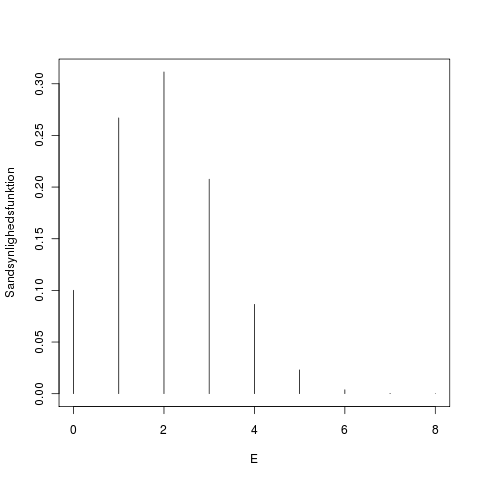
\includegraphics[width=0.5\textwidth]{8_plot_1}
        \label{binom_8}
    }
    \subfloat[$n = 20$ og $p = 0.25$]
        {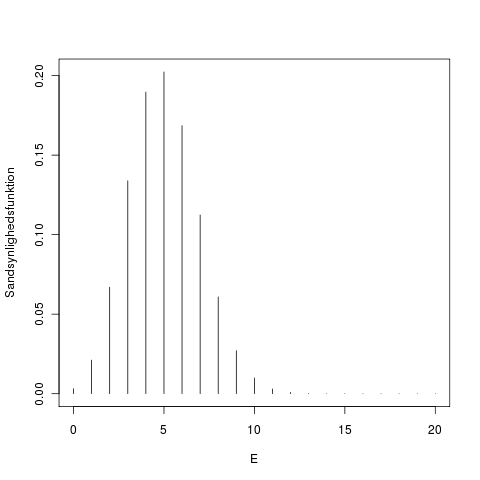
\includegraphics[width=0.5\textwidth]{20_plot_1}
        \label{binom_20}
    }\\
    \subfloat[$n = 100$ og $p = 0.25$]{
        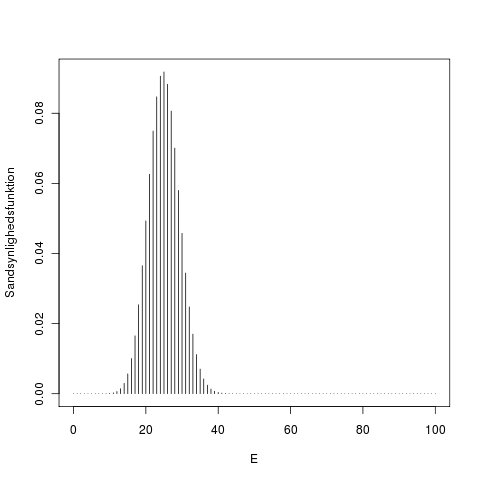
\includegraphics[width=0.5\textwidth]{100_plot_1}
        \label{binom_100}
    }
    \caption{Resultater fra binomialfordelinger med antalsparameter 8, 20
    og 100 og sandsynlighedsparameter $\frac{1}{4}$}
    \label{binom8_20_100}
\end{figure}

}


\section*{Opgave 2}
{
% Indsæt lort
}


\section*{Opgave 3}
{
\begin{verbatim}
[1] Mean for simulation with size 8 is: 2.029
[1] Var for simulation with size 8 is: 1.60376276276276
[1]
[1] Mean for simulation with size 20 is: 4.997
[1] Var for simulation with size 20 is: 3.55654754754755
[1]
[1] Mean for simulation with size 100 is: 25.087
[1] Var for simulation with size 100 is: 17.6550860860861
\end{verbatim}
}


\section*{Opgave 4}

\section*{Opgave 5}
{
Vi får at vide, at binomialfordelingen tilnærmer sig normalfordelingen
for store værdier af $n$. Dette ses i figur \ref{hist8_20_100}. For
$n = 8$ ses det at de observerede værdier fra simulationen ikke følger
normalfordelingen. Ved $n = 20$ ligger vi tættere på normalfordelingen.
For $n = 100$ ligger observationerne stort set på niveau med
normalfordelingen, men vi lægger også her mærke til at der i intervallet
$[24,26)$ er et højt antal observationer, som vi så i opgave 2. Også
intervallet $[30,32)$ ligger udenfor normalfordelingen, men her er der et
færre antal observationer.

\begin{figure}[!h]
    \centering
    \subfloat[$n = 8$ og $p = 0.25$]{
        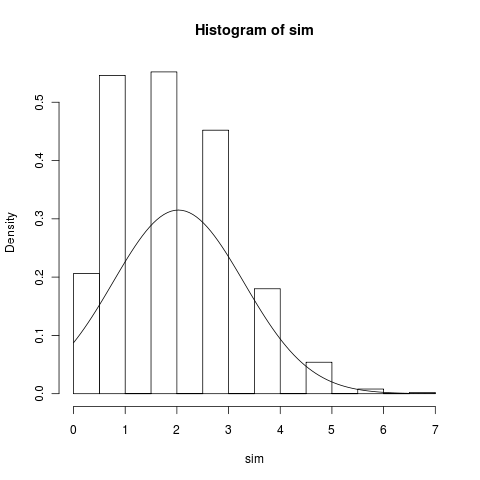
\includegraphics[width=0.5\textwidth]{8_hist_5}
        \label{hist_8}
    }
    \subfloat[$n = 20$ og $p = 0.25$]
        {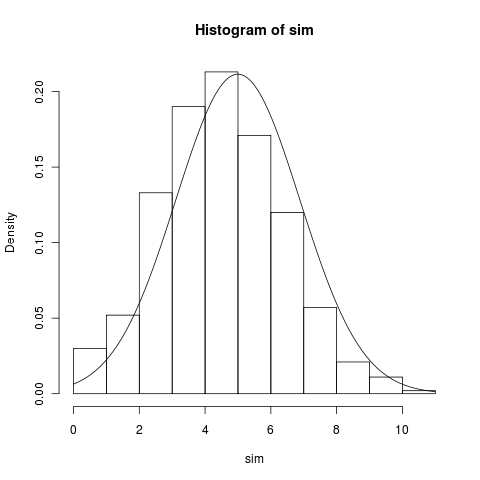
\includegraphics[width=0.5\textwidth]{20_hist_5}
        \label{hist_20}
    }\\
    \subfloat[$n = 100$ og $p = 0.25$]{
        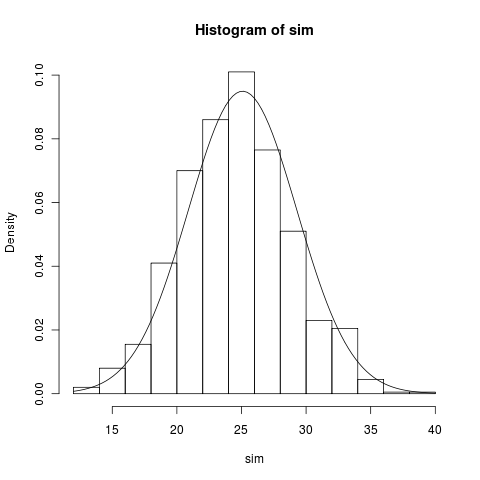
\includegraphics[width=0.5\textwidth]{100_hist_5}
        \label{hist_100}
    }
    \caption{Histogram og normalfordeling}
    \label{hist8_20_100}
\end{figure}

}


\section*{Opgave 6}

\section*{Opgave 7}

\section*{Opgave 8}

\section*{Opgave 9}
\newpage

%%%%%%%%%%%%%%%%%%%%%%%%%%%%%%%%%%%%%%%%%%%%%%%%%%%%%%%%%%%%%%%
% Bilag
\appendix

\section{Source code}
\subsection{main.r \label{app_source1}}
\lstinputlisting{../src/main.r}

\end{document}
